\documentclass[11pt,a4paper]{article}
\usepackage[margin=2.2cm]{geometry}
\usepackage{times}
\usepackage{amsmath,amssymb}
\usepackage{booktabs,tabularx,longtable}
\usepackage{graphicx}
\usepackage[hidelinks]{hyperref}
\usepackage{enumitem}
\usepackage[most]{tcolorbox}
\usepackage{titlesec}
\usepackage{fancyhdr}
\setlist{itemsep=2pt,topsep=3pt,leftmargin=*}
\graphicspath{{../../results/figures/}}
% generated by paper/make_values.py -- do not edit
\newcommand{\aucG}{0.539}
\newcommand{\aucGHi}{0.557}
\newcommand{\aucGLo}{0.521}
\newcommand{\aucGSd}{0.002}
\newcommand{\aucLenC}{0.542}
\newcommand{\aucLenCHi}{0.561}
\newcommand{\aucLenCLo}{0.524}
\newcommand{\aucLenCSd}{0.002}
\newcommand{\aucPA}{0.564}
\newcommand{\aucPAHi}{0.582}
\newcommand{\aucPALo}{0.545}
\newcommand{\aucPASd}{0.006}
\newcommand{\aucPB}{0.589}
\newcommand{\aucPBHi}{0.607}
\newcommand{\aucPBLo}{0.571}
\newcommand{\aucPBSd}{0.005}
\newcommand{\aucPC}{0.600}
\newcommand{\aucPCHi}{0.619}
\newcommand{\aucPCLo}{0.582}
\newcommand{\aucPCSd}{0.004}
\newcommand{\aucQ}{0.561}
\newcommand{\aucQG}{0.588}
\newcommand{\aucQGHi}{0.607}
\newcommand{\aucQGLo}{0.570}
\newcommand{\aucQGPA}{0.593}
\newcommand{\aucQGPAHi}{0.611}
\newcommand{\aucQGPALo}{0.575}
\newcommand{\aucQGPASd}{0.004}
\newcommand{\aucQGPB}{0.610}
\newcommand{\aucQGPBHi}{0.628}
\newcommand{\aucQGPBLo}{0.592}
\newcommand{\aucQGPBSd}{0.004}
\newcommand{\aucQGPC}{0.619}
\newcommand{\aucQGPCHi}{0.637}
\newcommand{\aucQGPCLo}{0.601}
\newcommand{\aucQGPCSd}{0.003}
\newcommand{\aucQGSd}{0.003}
\newcommand{\aucQHi}{0.578}
\newcommand{\aucQLo}{0.543}
\newcommand{\aucQSd}{0.005}
\newcommand{\codeFlawed}{24}
\newcommand{\codeLowEnt}{6}
\newcommand{\codeN}{40}
\newcommand{\codeNotLoad}{5}
\newcommand{\codeQuest}{1}
\newcommand{\codeRepair}{4}
\newcommand{\dIncA}{+0.005}
\newcommand{\dIncAHi}{+0.014}
\newcommand{\dIncALo}{-0.004}
\newcommand{\dIncAP}{0.296}
\newcommand{\dIncB}{+0.022}
\newcommand{\dIncBHi}{+0.031}
\newcommand{\dIncBLo}{+0.011}
\newcommand{\dIncBP}{0.001}
\newcommand{\dIncC}{+0.031}
\newcommand{\dIncCHi}{+0.041}
\newcommand{\dIncCLo}{+0.020}
\newcommand{\dIncCP}{0.001}
\newcommand{\dPAvsQG}{-0.025}
\newcommand{\dPAvsQGHi}{-0.004}
\newcommand{\dPAvsQGLo}{-0.046}
\newcommand{\dPAvsQGP}{0.012}
\newcommand{\fatAll}{0.765}
\newcommand{\fatAllHi}{0.782}
\newcommand{\fatAllLo}{0.748}
\newcommand{\fatGsm}{0.966}
\newcommand{\fatGsmHi}{0.990}
\newcommand{\fatGsmLo}{0.942}
\newcommand{\fatLast}{0.890}
\newcommand{\fatMath}{0.842}
\newcommand{\fatMathHi}{0.869}
\newcommand{\fatMathLo}{0.814}
\newcommand{\fatOly}{0.756}
\newcommand{\fatOlyHi}{0.788}
\newcommand{\fatOlyLo}{0.725}
\newcommand{\fatOmni}{0.659}
\newcommand{\fatOmniHi}{0.692}
\newcommand{\fatOmniLo}{0.624}
\newcommand{\fatOnsetMax}{0.766}
\newcommand{\fatOnsetMin}{0.749}
\newcommand{\fatPredErrStep}{0.670}
\newcommand{\fatPredMaxInc}{0.003}
\newcommand{\fatPredPos}{0.484}
\newcommand{\fatPredQG}{0.671}
\newcommand{\lenFixA}{+0.052}
\newcommand{\lenFixAP}{0.032}
\newcommand{\markFat}{15.5}
\newcommand{\markP}{0.09}
\newcommand{\markRec}{18.6}
\newcommand{\mwRhoP}{0.21}
\newcommand{\mwRhoR}{0.04}
\newcommand{\nErr}{2,221}
\newcommand{\nFatal}{1,700}
\newcommand{\nRecovered}{521}
\newcommand{\nonFatalOmniPct}{34.1}
\newcommand{\nonFatalPct}{23.5}
\newcommand{\twErrFC}{0.709}
\newcommand{\twErrFCHi}{0.726}
\newcommand{\twErrFCLo}{0.691}
\newcommand{\twErrFR}{0.376}
\newcommand{\twErrFRHi}{0.402}
\newcommand{\twErrFRLo}{0.350}
\newcommand{\twErrRC}{0.819}
\newcommand{\twErrRCHi}{0.840}
\newcommand{\twErrRCLo}{0.796}
\newcommand{\twOutFC}{0.664}
\newcommand{\twOutFCHi}{0.683}
\newcommand{\twOutFCLo}{0.645}
\newcommand{\twOutFR}{0.456}
\newcommand{\twOutFRHi}{0.484}
\newcommand{\twOutFRLo}{0.428}
\newcommand{\twOutQGFC}{0.672}
\newcommand{\twOutQGFCHi}{0.692}
\newcommand{\twOutQGFCLo}{0.653}
\newcommand{\twOutQGFR}{0.501}
\newcommand{\twOutQGFRHi}{0.526}
\newcommand{\twOutQGFRLo}{0.473}
\newcommand{\twOutQGRC}{0.679}
\newcommand{\twOutQGRCHi}{0.706}
\newcommand{\twOutQGRCLo}{0.650}
\newcommand{\twOutRC}{0.703}
\newcommand{\twOutRCHi}{0.729}
\newcommand{\twOutRCLo}{0.677}
\newcommand{\wpG}{0.548}
\newcommand{\wpGHi}{0.591}
\newcommand{\wpGLo}{0.504}
\newcommand{\wpPA}{0.485}
\newcommand{\wpPAHi}{0.536}
\newcommand{\wpPALo}{0.440}
\newcommand{\wpPC}{0.539}
\newcommand{\wpPCHi}{0.589}
\newcommand{\wpPCLo}{0.487}
\newcommand{\wpPairs}{466}
\newcommand{\wpProblems}{326}
\newcommand{\wpQGPC}{0.586}
\newcommand{\wpQGPCHi}{0.634}
\newcommand{\wpQGPCLo}{0.535}

\definecolor{acc}{HTML}{2a78d6}
\definecolor{warn}{HTML}{eb6834}
\definecolor{ok}{HTML}{1baf7a}
\titleformat{\section}{\Large\bfseries\color{acc}}{\thesection}{0.6em}{}
\titleformat{\subsection}{\large\bfseries}{\thesubsection}{0.5em}{}
\newtcolorbox{viva}[1][]{colback=acc!5,colframe=acc,fonttitle=\bfseries,title={#1},left=6pt,right=6pt,top=4pt,bottom=4pt}
\newtcolorbox{plain}[1][]{colback=ok!6,colframe=ok,fonttitle=\bfseries,title={#1},left=6pt,right=6pt,top=4pt,bottom=4pt}
\newtcolorbox{caution}[1][]{colback=warn!6,colframe=warn,fonttitle=\bfseries,title={#1},left=6pt,right=6pt,top=4pt,bottom=4pt}
\pagestyle{fancy}\fancyhf{}
\rhead{\small Errors Are Not Choke Points: the research story}\lhead{\small MSE-2 guide}\cfoot{\thepage}
\setlength{\parskip}{4pt}\setlength{\parindent}{0pt}

\begin{document}
\begin{titlepage}
\centering
\vspace*{2cm}
{\Huge\bfseries Errors Are Not Choke Points\par}
\vspace{0.4cm}
{\Large Counterfactual localisation of LLM reasoning failures,\\[2pt] and why restart is hard to beat\par}
\vspace{1.2cm}
{\Large\bfseries The research story, start to finish\par}
{\large and a guide to the MSE-2 evaluation\par}
\vspace{1.5cm}
{\large Harsh Dubey \quad Harshit Saini \quad Prashant Jain\\[2pt]
Himanshu Kumar \quad Gaurav Kaushal \quad Rohit Chaudhary (supervisor)\par}
\vspace{0.5cm}
{Department of CSE (AI\&ML), KIET Group of Institutions, Ghaziabad\par}
\vspace{1.5cm}
\begin{tcolorbox}[colback=acc!5,colframe=acc,width=0.9\textwidth]
\textbf{How to use this document.} It tells what the project did, why, and what came out, in the
order it happened. Each part of the MSE-2 evaluation has its own section, so you can open the one
being asked about:\\[4pt]
\begin{tabularx}{\linewidth}{lXr}
\toprule
MSE-2 criterion & Where & Marks\\\midrule
Project: Model Training & Section~\ref{sec:training} & 5\\
Project: Hyperparameter Tuning & Section~\ref{sec:tuning} & 5\\
Project: Result Analysis & Section~\ref{sec:analysis} & 5\\
Research paper: Methodology & Section~\ref{sec:method} & 2.5\\
Research paper: Results & Section~\ref{sec:results} & 2.5\\\bottomrule
\end{tabularx}\\[4pt]
Every number in this guide is printed from the same generated file as the paper
(\texttt{paper/values.tex}, written by \texttt{paper/make\_values.py} from the result tables), so
the guide and the paper cannot disagree. Blue boxes give the one-line answer to say in the viva.
\end{tcolorbox}
\vfill
{\small Status: preprint draft, October 2026. Code and data: \texttt{github.com/HarshDubey23/early-failure-detection-cot}}
\end{titlepage}

\tableofcontents
\newpage

%==========================================================================================
\section{The whole project in one page}\label{sec:onepage}

\textbf{The goal.} Reduce the failures of large language models (LLMs): wrong answers in
step-by-step maths and hallucinations (claims not supported by the source) in retrieval-augmented
generation (RAG), at the lowest possible cost.

\textbf{The popular idea we tested.} Most methods are \emph{surgical}: find the step where the output
went wrong, go back to just before it, and repair or regenerate from there. Process reward models
(PRMs) are trained to find that step; hallucination-repair systems do the same for unsupported
sentences. It sounds efficient, because it keeps the good part of the answer.

\textbf{The one quantity.} For a solution written by model $M$, let
\[ v_k = P_M(\text{correct final answer} \mid \text{question and the first } k \text{ steps}). \]
We estimate $v_k$ by letting $M$ itself continue from step $k$ many times and counting how often it
ends up correct. $v_0$ is ``solve from scratch''. Resampling from $k=0$ is a \emph{restart};
resampling from just before step $j$ is \emph{backtracking}. The step where $v$ collapses is the
\emph{choke point}; the step a human marks as the first mistake is the \emph{error}.

\textbf{Main finding: errors are not choke points, and restart is hard to beat.}
\begin{enumerate}
\item Early-warning detectors mostly measure how hard the question is: question and model alone
reach AUROC \aucQG; the first quarter of the reasoning adds \dIncA\ (not significant).
\item \QwenSmallAllCapPct--\QwenMathCapPct\% of failures are decided before the first step. When the
outcome is still open, the human-marked error is the choke point in \QwenTwoAllDec--\QwenSmallAllDec\
of traces, against a chance level of about 0.18 (preregistered, confirmed on Llama-3.1-8B).
\item A PRM finds the human-marked error \cbPrmDropAccHPct\% of the time but the choke point only
\cbPrmDropAccDPct\% (ChokeBench v1, our new benchmark and evaluation protocol, \cbN\ failed traces). A model we trained and tuned for the choke point
does no better (\cbLearnedAccD).
\item ChokeBench predicts real recovery. With the choke point labelled on one half of the samples
and gains scored on the other, naming the choke point raises a trace's recovery gain by \valBothD,
while the human label adds only \valBothE\ once the choke point is accounted for. On a held-out
model, ChokeBench scores rank localisers by their actual gain with Spearman \valRhoD, against
\valRhoE\ for first-error scores (exploratory).
\item No deployable choice of where to resample reliably beats a plain restart at equal compute. Even
a free, perfect choke-point oracle gains only \cbOracleGainB\ at four restarts' budget; in RAG,
choosing where to resample adds \rrHFive.
\item Plain restarting recovers \recMinFour--\recMaxFour\% of failed maths solutions within four
attempts' compute (\recMinEight--\recMaxEight\% within eight). It is the baseline any
localise-and-repair method must beat.
\item Run D, reasoning models with exactly on-policy traces: accuracy \rdQwenAcc\% (Qwen3-1.7B) and
\rdROneAcc\% (R1-distill), and over 90\% of failures are budget exhaustion. On R1-distill, no cut of a
failed trace is worth more than a fresh start (down to \rdDOneLast\ at 5,120 tokens), as Proposition 1
predicts. At matched compute the preregistered estimator gives the best cut \rdDTwo\ over restart, but only
through cheaper late attempts, and a plug-in check gives \rdDTwoPlug\ (n.s.).
\end{enumerate}
\textbf{Secondary study: RAG hallucinations (LLM graders only, human ratings pending).}
\begin{enumerate}[resume]
\item A detector-gated resampling loop lowers the \emph{judged} hallucination rate by \rrHZero\
(preregistered, $p=\rrHZeroP$), but the judge agrees only weakly with people ($\kappa=\evEOneKappa$).
Plain detect--restart--abstain matches the choke-point-aware controller (\rrHOne) at \costDra$\times$
the base cost, against \costCare$\times$.
\item A short proposition says a restart loop's delivered hallucination rate is the detector's
$P(\text{hallucinated}\mid\text{pass})$, whatever the retry budget; from human labels of drafts it
predicts \lawH\% $\to$ \lawPi\%. This is a prediction, not yet a measurement on outputs.
\item The measured benefit depends on who grades it: \robBaseETwoDiff\ by a grader trained like the
detector, \robBaseEOneDiff\ (n.s.) by an independent one.
\end{enumerate}

\begin{figure}[h]\centering
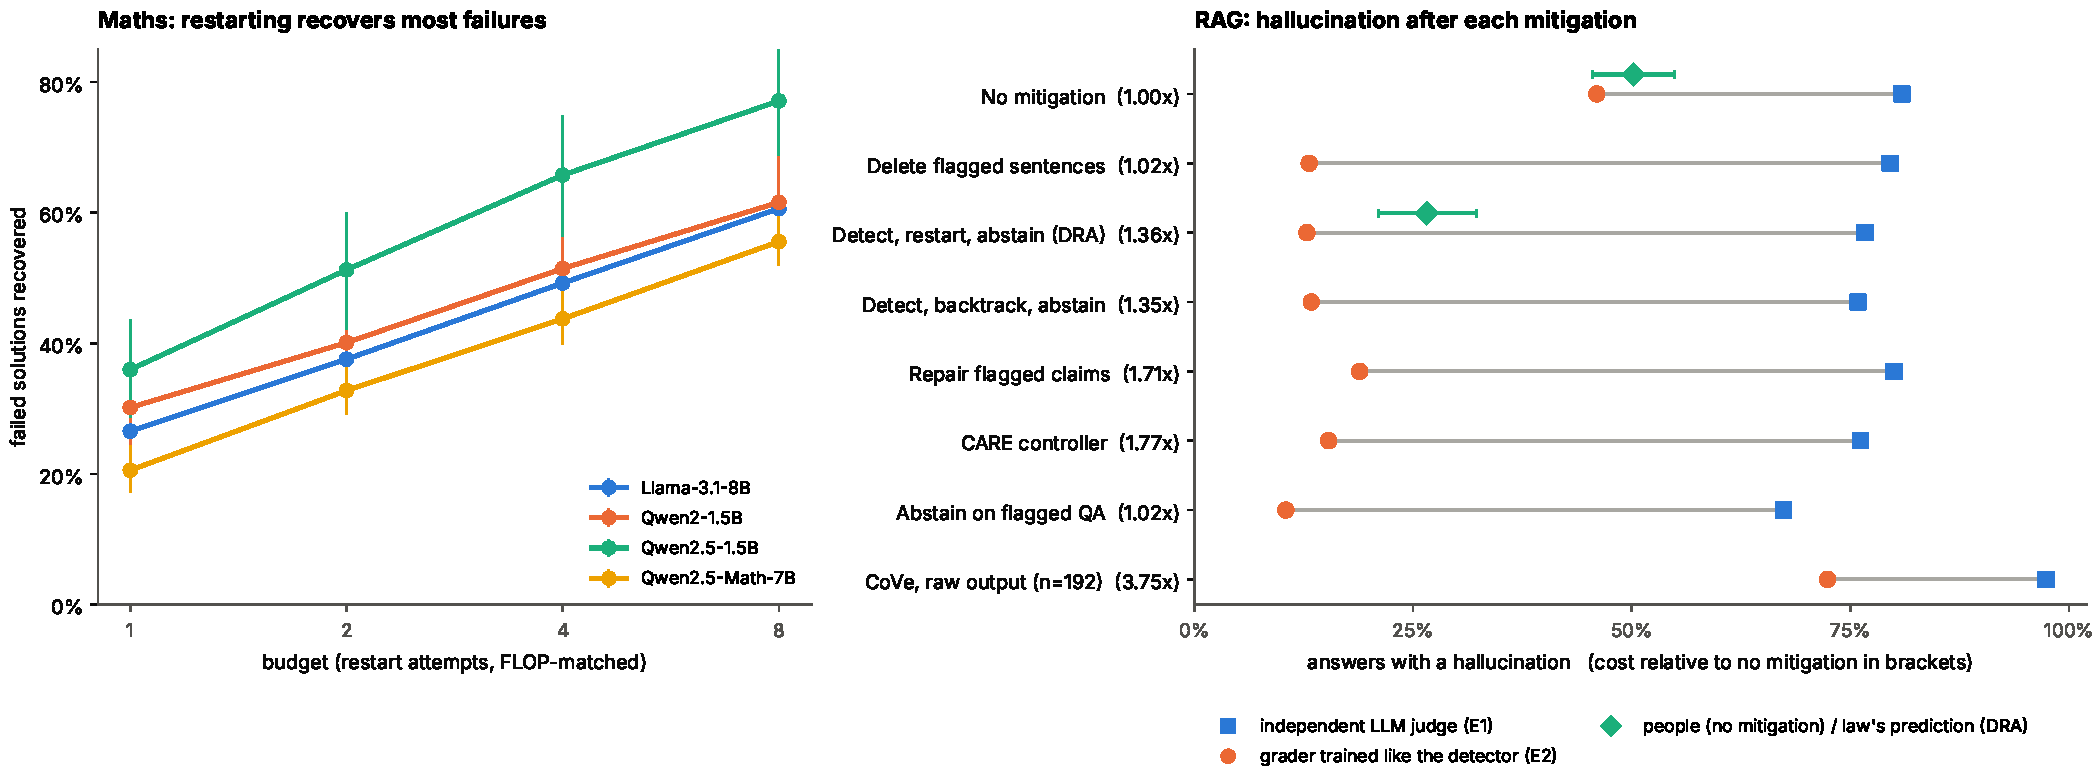
\includegraphics[width=\textwidth]{fig27_mitigation.pdf}
\caption{What mitigation buys: failed maths solutions recovered by restarting (left) and
hallucination after each RAG mitigation, with its cost (right).}
\end{figure}

\begin{figure}[h]\centering
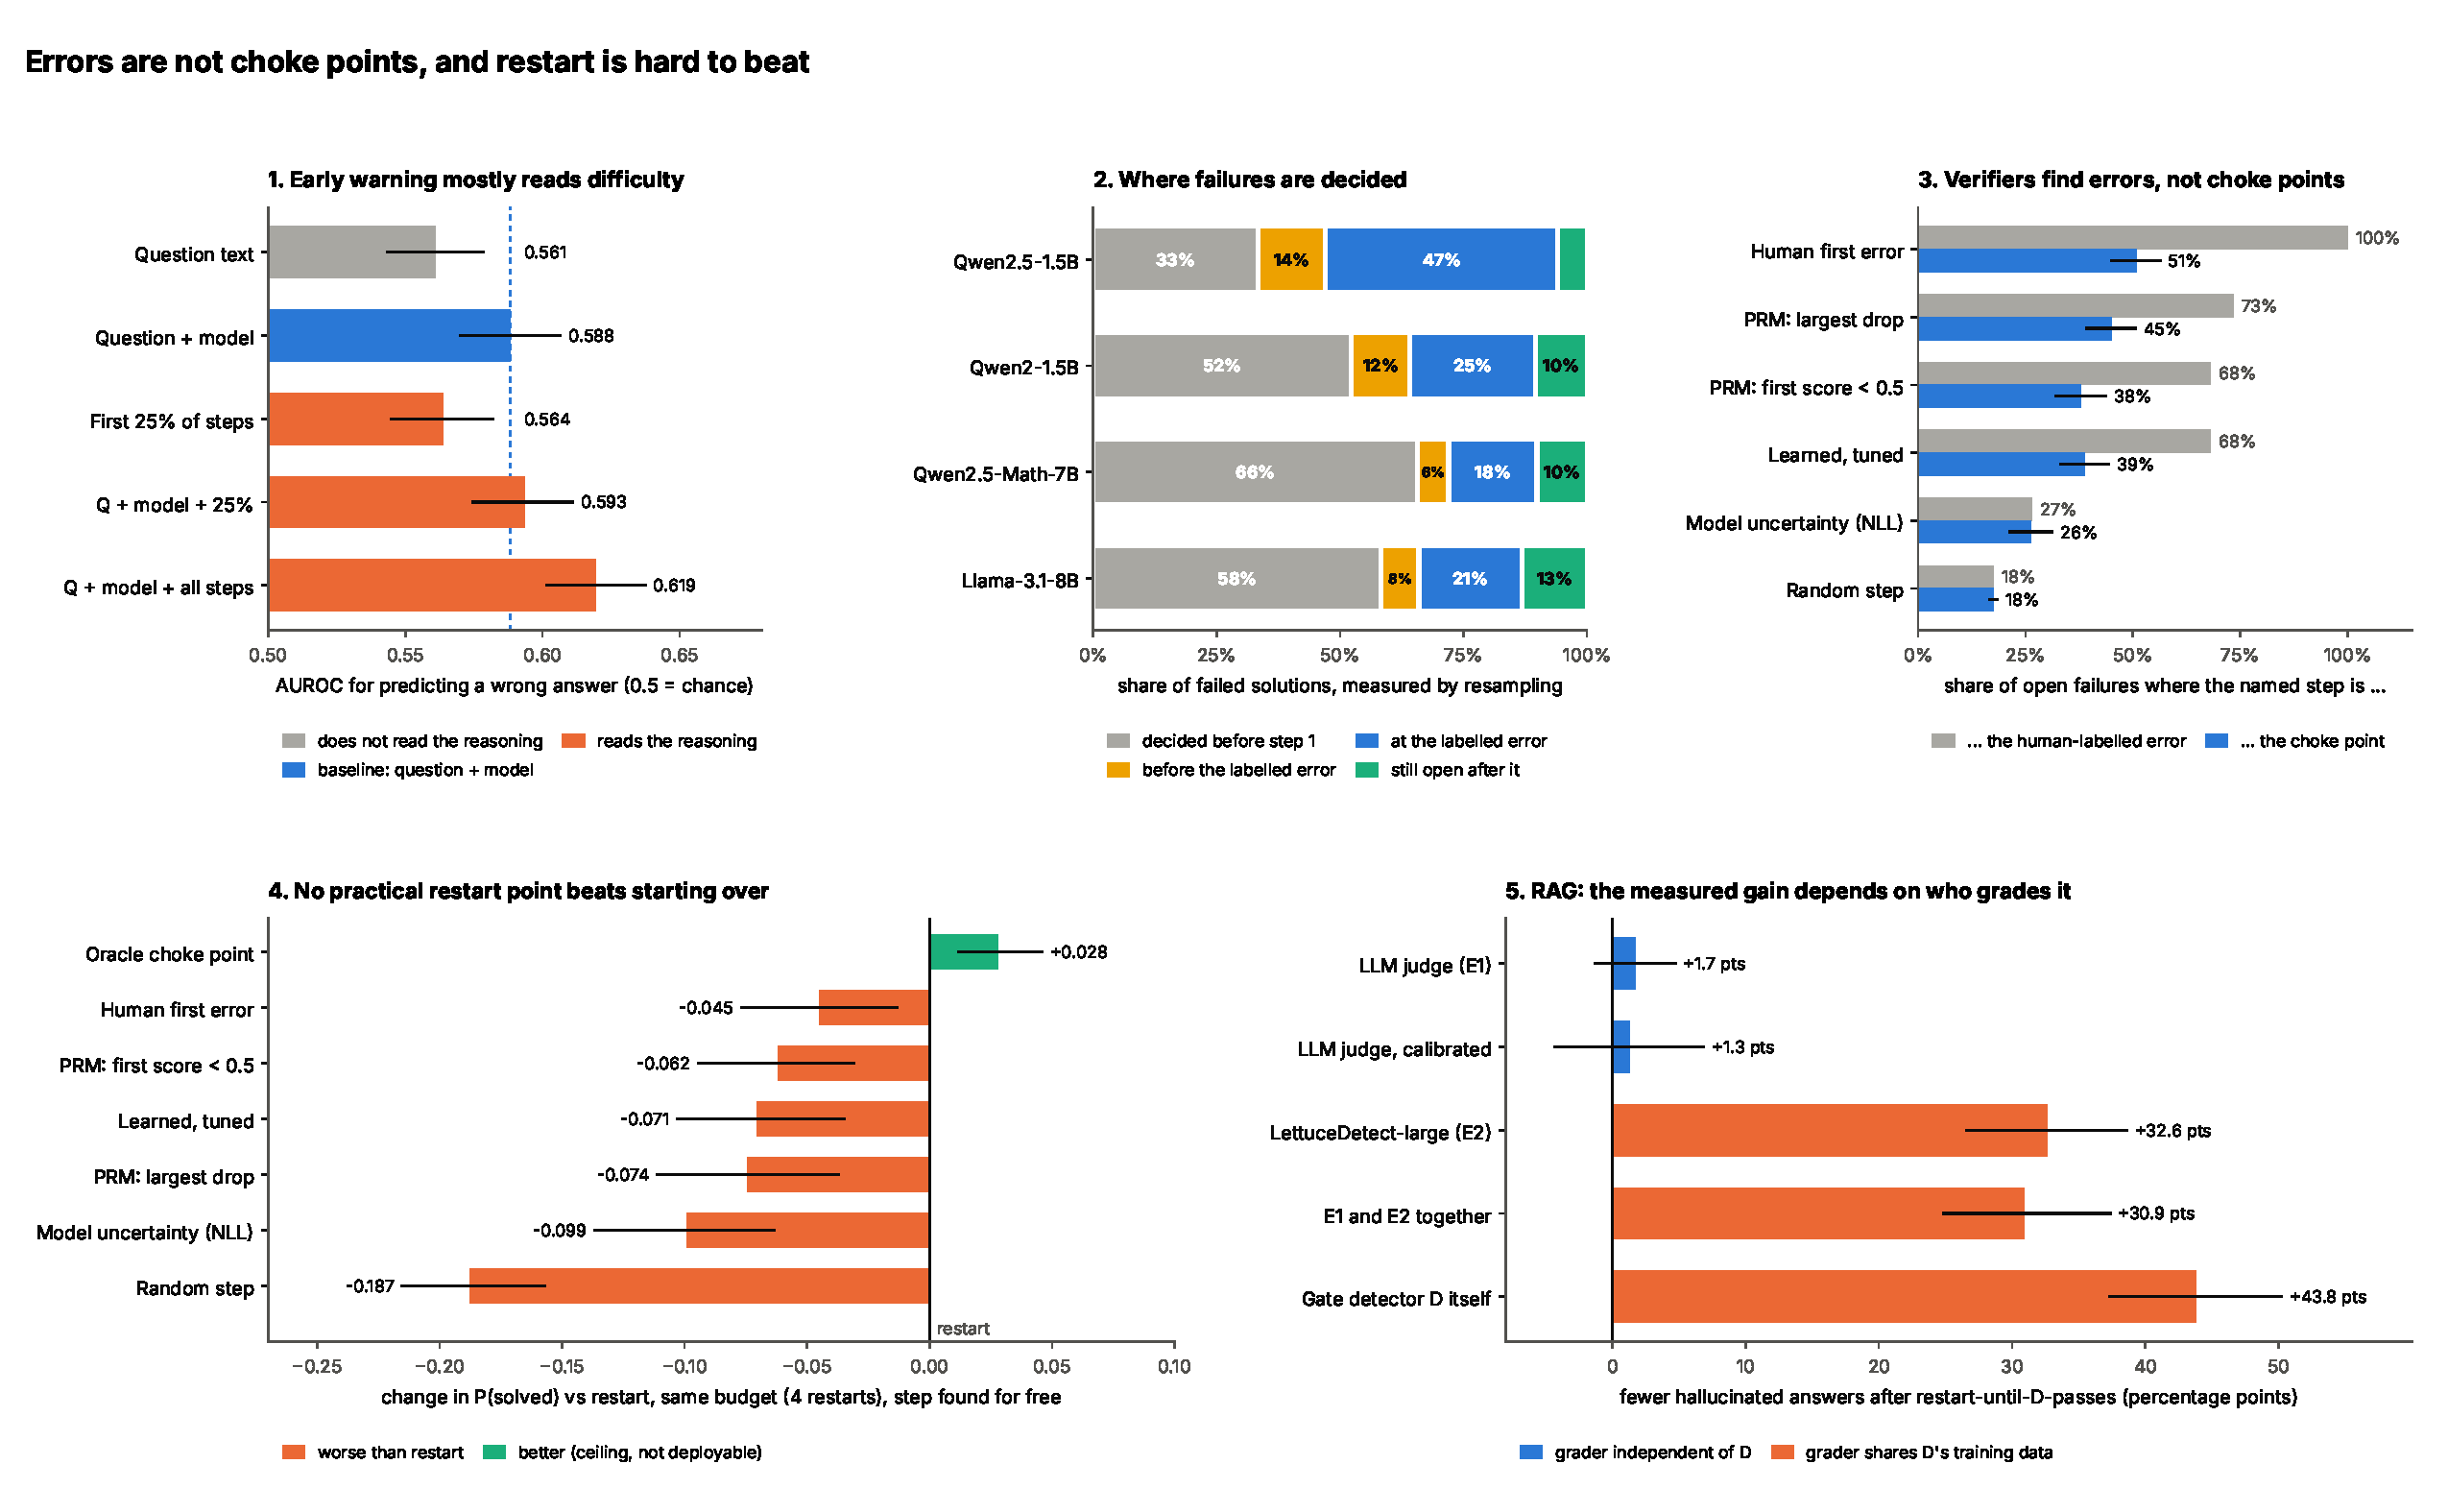
\includegraphics[width=\textwidth]{fig0_story.pdf}
\caption{Why the surgical version does not pay. Each panel is one of findings 3--7.}
\end{figure}

\begin{viva}[If you get one sentence]
``To reduce LLM failures and hallucinations cheaply, detect them and restart, abstaining if still
unsafe; we prove the result is only as good as the detector, and show by resampling the model itself
that the popular alternative, finding the bad step and repairing from there, does not beat
restarting at equal compute, because failures are rarely decided where we can see them.''
\end{viva}

%==========================================================================================
\section{How the project unfolded}\label{sec:timeline}

Research rarely goes in a straight line. This one changed direction twice, and both changes made
it stronger. The dates come from the git history.

\begin{longtable}{p{2.1cm}p{13.4cm}}
\toprule
When & What happened and why\\\midrule
15 Sep 2026 & \textbf{Original study (E1--E8).} Question: can a partial chain of thought predict a
wrong final answer, and where do first errors occur? Data: ProcessBench (3,400 maths solutions from
12 models, with the expert-marked first wrong step). We trained detectors (TF-IDF + logistic
regression, a surface-feature MLP and a GRU) on growing prefixes of each solution. Result: the
lexical detector reached AUROC 0.588 at 25\% of the chain and 0.626 on the whole chain.\\
24 Oct & \textbf{Novelty audit and first pivot.} A literature check showed two problems: (i) other
groups had already predicted success from hidden states, and (ii) a detector that never reads the
reasoning (question text + which model wrote it) also reaches 0.588. So the ``early warning'' was
mostly a \emph{difficulty} signal. We added difficulty controls and asked a sharper question:
is the human-marked first error the point where the outcome is decided?\\
24 Oct & \textbf{Runs A and B (GPU, Kaggle).} We built the counterfactual pipeline: for every prefix
of a solution, sample the same model many times and estimate $v_k$. Pilot (Run A) checked noise;
Run B covered three Qwen models. The hypotheses H1--H4 were written down and committed
\emph{before} any rollout (commit \texttt{a6fb04c}).\\
24--25 Oct & \textbf{Preregistered confirmatory Run C.} Before collecting new data we committed a
second plan (\texttt{459ff22}): tests C1--C4 on a new model family (Llama-3.1-8B), replication
R1--R3 on fresh sampling batches, and practical policies with full compute accounting. Some tests
were confirmed and some failed; both are reported.\\
25--26 Oct & \textbf{Run R: hallucinations.} We asked whether the same holds for RAG. We built a
recovery controller (CARE) that detects a hallucinated sentence and chooses between repairing it,
backtracking and restarting by estimated recoverability, preregistered its test, and ran it on
RAGTruth and HotpotQA with Llama-2-7B. Two bugs found during the run (a chat preamble corrupting
repairs, and CoVe echoing its verification block) were fixed and documented.\\
26 Oct & \textbf{A wrong turn.} A ``dual consensus judge'' and a ``1,500-item generalisation'' table
were added in a hurry. They looked impressive but were not sound (Section~\ref{sec:integrity}).\\
27 Oct & \textbf{Corrections and the final contributions.} We withdrew those claims, rebuilt the
paper from the tables, fixed the references, and added three CPU analyses on the existing data:
ChokeBench, a learned and tuned choke-point localiser, and a five-grader robustness check of Part 3.
This is the version in the final draft.\\
27 Oct (evening) & \textbf{Reframed around mitigation.} The results answer the original goal,
reducing failures and hallucinations, more directly than the title said: detect, restart and abstain
is the cheapest mitigation that works, and we added its law with a proof and a cost comparison of every
mitigation. The paper was titled \emph{Detect, Restart, Abstain}.\\
27 Oct (night) & \textbf{External review and refocus.} A critical review made five points, and we
accepted them. Early detection is a negative result. The paper tried to sell five contributions at
once. The RAG gain rests on an LLM judge with $\kappa=\evEOneKappa$ and has no human ratings yet.
ChokeBench is a first resource, not an established standard. And counterfactual resampling itself
is prior work. The main contribution is now the counterfactual localisation and compute-matched
recovery result, and RAG is a clearly secondary study. The paper is now titled \emph{Errors Are Not
Choke Points}.\\\bottomrule
\end{longtable}

\begin{plain}[Why the pivot matters (good viva point)]
The first version answered an easier question with a confound we had not controlled. Adding a
question-only baseline exposed it. Turning a weak result into a sharp new question, and
preregistering the test of it, is what turned a course project into a research paper.
\end{plain}

%==========================================================================================
\section{Background in plain words}\label{sec:background}

\begin{description}
\item[Chain of thought (CoT).] The model writes its reasoning as numbered steps before the answer.
\item[Process reward model (PRM).] A second model that scores each step as right or wrong. We use
Qwen2.5-Math-PRM-7B.
\item[First error $e$.] The first step a human expert marks as wrong (ProcessBench labels).
\item[$v_k$ and the choke point $d$.] $v_k$ is defined above; $d=\arg\max_k (v_{k-1}-v_k)$, the step
with the largest fall in the chance of success.
\item[Capability-limited.] The model solves the question from scratch at most one time in eight
($v_0\le\delta=1/8$). Then no step is a choke point: the failure was decided before the first step.
\item[Restart vs backtrack.] Start again from the question, or resample from just before step $j$.
\item[Matched compute.] Every method gets the same token budget, counted in ``restart attempts'',
including the cost of running the verifier.
\item[AUROC.] Probability that a detector ranks a random failing solution above a random correct
one. 0.5 is chance, 1.0 is perfect.
\item[Cohen's $\kappa$.] Agreement between two raters beyond chance. 0 is chance, 1 is perfect.
\item[Bootstrap CI.] Resample the data with replacement many times and read the 2.5th and 97.5th
percentiles of the estimate. We resample whole questions or traces, not rows (cluster bootstrap).
\item[Preregistration.] Writing the hypotheses and analysis into the git history before the data
exist, so results cannot be cherry-picked afterwards.
\item[RAG.] Retrieval-augmented generation: the model answers from given source passages. A
\emph{hallucination} is a sentence the source does not support.
\end{description}

%==========================================================================================
\section{Methodology}\label{sec:method}
\begin{viva}[Research paper: Methodology (2.5 marks)]
Three studies connected by one measurement, $v_k$. Data with human error labels; on-policy
resampling to measure where outcomes are decided; matched-compute comparison of recovery policies;
preregistered tests with cluster-bootstrap CIs; every number generated by code.
\end{viva}

\subsection{Data}
\begin{itemize}
\item \textbf{ProcessBench}: 3,400 step-by-step solutions to GSM8K, MATH, OlympiadBench and
Omni-MATH problems (2,842 distinct problems), written by 12 open models, each with the expert first
error and whether the final answer is correct. Correct and incorrect answers are balanced.
\item \textbf{RAGTruth} test sources (450): Llama-2-7B-chat answers for QA, summarisation and
data-to-text, with human-marked hallucinated spans. \textbf{HotpotQA}: 300 items with controlled
evidence (half have the answer removed, to test abstention).
\end{itemize}

\subsection{Part 1: is early warning a difficulty signal?}
Detectors read either the question text (Q), the generator and tier (G), a prefix of the reasoning,
or combinations. TF-IDF (uni- and bigrams) or one-hot features feed a logistic regression,
\emph{cross-fitted over 5 folds grouped by problem} (a problem never appears in both training and
test) and repeated over 5 seeds. We report AUROC, the \emph{increment} of the reasoning over Q+G, and
a \emph{within-problem} concordance: for problems that have both a failing and a succeeding trace,
how often the detector ranks the failing one higher. Within a problem, difficulty is held fixed.

\subsection{Part 2: counterfactual commitment}
For every prefix $s_{1:k}$ ($k=0,\dots,n-1$) we sample $m$ continuations from the \emph{same model that
wrote the trace} (on-policy) with vLLM at temperature 0.7 and top-$p$ 0.95, and check the final
answer against the gold answer with \texttt{math-verify}. $m=\QwenSmallAllM$ for the 1.5B models
(four independent batches of 16), \QwenMathM\ for Qwen2.5-Math-7B and \LlamaM\ for Llama-3.1-8B:
\TotalRollouts\ continuations in total. Each failed trace is then classified as capability-limited,
latent commitment (collapse before the marked error), commits at the error, or recoverable error.
Three safeguards:
\begin{itemize}
\item \textbf{Position-matched null}: how often a randomly placed ``error'' would coincide with the
choke point, given each trace's length.
\item \textbf{Sample splitting}: one half of the continuations chooses the choke point, the other
half scores it, over 50 random splits; otherwise noise would be rewarded.
\item \textbf{Reliability}: correlation of $v_k$ between independent batches, and a Bayesian
(Jeffreys) posterior over the choke point (2,000 draws).
\end{itemize}

\subsection{Recovery policies at matched compute}
Restart; PRM first step below 0.5; PRM largest drop; probe search; a learned restart point; the
human first error and the oracle choke point as references. Cost counts every token, weighted by
model size (FLOPs $\propto$ parameters $\times$ tokens): prefill once per restart point, every
generated token, every PRM pass and probe. With budget $b$ restart attempts, a policy spends what
is left after its overhead on independent attempts from its restart point; we report P(at least one
correct).

\subsection{ChokeBench (new)}
A benchmark that grades a step localiser on two targets: the human first error and the choke point,
and on what the named step is worth as a resampling point (per attempt, and at a 4$\times$ budget with
localisation free, which upper-bounds any verifier).

\subsection{Part 3: recovery from hallucinations}
The controller CARE gates on detector $D$ (LettuceDetect-base). When $D$ flags a sentence: repair
the claim, then resample, choosing restart or backtrack by Thompson sampling on each boundary's
recoverability per token, then abstain (QA) or delete what is still flagged. Every policy replays the
same bank of continuations under a budget cap of 2. The primary grader $E_1$ is an LLM judge from
another family (Qwen2.5-7B-Instruct), validated against RAGTruth's human labels before reading any
comparison; $E_2$ (LettuceDetect-large) is secondary.

\subsection{Statistics and evidence levels}
95\% cluster-bootstrap CIs (1,000--2,000 resamples); paired differences on the same items;
sign-flip permutation p-values with Holm correction for multiple tests; TOST for equivalence
(``no difference'' is never written as ``equal'' unless TOST passes). Every claim carries a label:
\textsc{pre} (preregistered), \textsc{exp} (exploratory), \textsc{conf} (preregistered test on new data).

\subsection{Theory: three propositions}
\textbf{Proposition 1 (a failed prefix is worth no more than a fresh start).}
Under the model's own sampling, $v_k$ is a martingale (on average it neither rises nor falls). For
any rule that picks the restart point by reading the trace only up to that point,
\[ \mathbb{E}[v_\tau \mid \text{fail}] = \frac{\mathbb{E}[v_\tau(1-v_\tau)]}{1-v_0} \le v_0 , \]
because $x(1-x)$ is concave. In words: averaged over failures, a failed trace cut at any point
chosen without looking ahead is worth no more than a fresh start. Backtracking can only win by
looking ahead (e.g.\ resampling from \emph{before} a flagged step) or by saving tokens.

%==========================================================================================
\textbf{Proposition 2 (shorter attempts are the only advantage).} If resampling from point $k$
succeeds no more often per attempt than restarting ($v_k\le v_0$), then with any budget it is worth at
most a restart given $c_0/c_k$ times the budget, where $c$ is the length of one attempt. Measured
lengths give $c_k/c_0\approx0.7$--$0.8$, so the best such point is worth at most 1.25--1.4 restarts'
budgets, before paying to find it.

\textbf{Proposition 3 (a restart loop is exactly as faithful as its detector).} Suppose the system
draws independent answers and returns the first one the detector passes, abstaining after $K+1$
flagged draws. With $h$ the hallucination rate of a draw, $\beta$ the detector's miss rate and
$\alpha$ its false-alarm rate,
\[ P(\text{hallucinated}\mid\text{answered}) = \frac{h\beta}{h\beta+(1-h)(1-\alpha)}, \qquad
P(\text{answered}) = 1-q^{K+1},\ q = h(1-\beta)+(1-h)\alpha . \]
\emph{Why:} every draw is independently ``passed and hallucinated'' ($h\beta$), ``passed and faithful''
($(1-h)(1-\alpha)$) or ``flagged'' ($q$); the loop returns the first passed draw, so whichever draw it
returns, the odds of hallucinated vs faithful are $h\beta : (1-h)(1-\alpha)$, the same at every try. So
more retries buy coverage, never faithfulness, and the place where we resample does not appear in
the formula at all. Plugging in the detector's error rates measured on RAGTruth's human labels
($\beta=\lawBeta\%$, $\alpha=\lawAlpha\%$, $h=\lawH\%$) predicts \lawPi\% [\lawPiLo, \lawPiHi]
hallucinated answers after DRA, a reduction of \lawRed\ points. Two assumptions carry this
(independent draws; the detector's errors on resampled answers equal those on drafts), so it is an
exploratory estimate until people rate the outputs.

\section{Model training}\label{sec:training}
\begin{viva}[Project: Model Training (5 marks)]
The large language models are used frozen; what we train are the decision models built on top of
them: failure detectors, a restart-point predictor and a choke-point localiser, always with
group-wise splits so no problem (or no model) leaks from training into testing.
\end{viva}

\subsection{What is frozen and what is trained}
\begin{longtable}{p{4.6cm}p{5.4cm}p{5.3cm}}
\toprule
Model & Role & Trained by us?\\\midrule
Qwen2.5-1.5B, Qwen2-1.5B, Qwen2.5-Math-7B, Llama-3.1-8B (instruct) & generators whose own continuations define $v_k$ & No: frozen. Training them would change the very thing we measure.\\
Llama-2-7B-chat & RAG generator & No (frozen)\\
Qwen2.5-Math-PRM-7B & step verifier & No; re-validated: ProcessBench F1 \prmFOne\ vs published 73.5\\
LettuceDetect base / large & hallucination detector / grader & No (frozen, trained by its authors on RAGTruth)\\
Qwen2.5-7B-Instruct & LLM judge $E_1$ & No; validated against human labels ($\kappa=\evEOneKappa$)\\\midrule
TF-IDF + logistic regression & failure detectors (Parts 1, E3) & \textbf{Yes}\\
Surface-feature MLP (64--32) and GRU (hidden 32) & failure detectors (E3) & \textbf{Yes}\\
Stepwise lexical detectors & one per step count, for lead time (E5) & \textbf{Yes}\\
Learned restart-point predictor (P4) & picks where to resample & \textbf{Yes}\\
Learned choke-point localiser & ChokeBench entry & \textbf{Yes} (with tuning, Section~\ref{sec:tuning})\\
Calibrated judge threshold & D-independent grader for Part 3 & \textbf{Yes} (threshold fit on DEV)\\\bottomrule
\end{longtable}

\subsection{How the failure detectors are trained (Parts 1 and E3)}
\begin{enumerate}
\item \textbf{Input.} A prefix of the solution: the first $k=\max(1,\lceil fn\rceil)$ steps for $f$ in a
grid from 10\% to 100\%; or the question text; or the generator's identity.
\item \textbf{Features.} TF-IDF of words and word pairs (at most 20,000 features, a term must appear in
at least 2 training prefixes), fitted on \emph{training prefixes only}; or surface features (step and
character counts, position), standardised with training statistics.
\item \textbf{Model.} L2-regularised logistic regression (or the MLP / GRU), target $y=1$ if the final
answer is wrong.
\item \textbf{Split.} Grouped by problem: 25\% of problems held out (E3), or 5-fold cross-fitting
grouped by problem, repeated with 5 seeds (Part 1). An automated test (\texttt{tests/test\_no\_leakage.py})
fails the build if any problem appears on both sides.
\end{enumerate}
\textbf{Why grouped splits matter.} 3,400 rows contain only 2,842 problems. A random row split would
put the same problem in training and test, and the detector would score well by memorising problems.

\subsection{How the learned restart-point predictor (P4) is trained}
Each step of a failed trace is one example with 8 features: PRM score and its drop, the generator's
mean and maximum token negative log-likelihood (NLL) and entropy, relative position and step length.
Label: 1 for the choke point chosen on half A of the continuations, 0 otherwise. Logistic regression on
standardised features, trained on the \emph{other} generators (for Llama: only on the three Qwen
models), so the test model is never seen. At test time the step with the highest probability is the
restart point.

\subsection{How the learned choke-point localiser is trained (new)}
\begin{itemize}
\item \textbf{Examples}: every step of the open failed traces of the training generators, nine
features (the eight above plus ``first PRM score below 0.5'').
\item \textbf{Soft labels}: instead of a hard 0/1 we use the posterior probability $P(d=j)$ that step $j$
is the choke point. Each step is entered twice, as label 1 with weight $P(d=j)$ and label 0 with weight
$1-P(d=j)$; weights are divided by the trace length so every trace counts once. This keeps sampling
uncertainty in the target instead of pretending the choke point is known exactly.
\item \textbf{Models}: logistic regression or gradient-boosted trees (scikit-learn).
\item \textbf{Evaluation}: leave-one-generator-out. The held-out model is never used for training or
for choosing hyperparameters.
\end{itemize}

\begin{caution}[What we did not train, and why]
We did not fine-tune any LLM. The research question is about how existing models and verifiers
behave; fine-tuning the generator would change $v_k$ itself. The hidden-state probes planned in the
first version (E4) were not run, because others had already published that result and the GPU budget
went to the counterfactual runs instead.
\end{caution}

%==========================================================================================
\section{Hyperparameter tuning}\label{sec:tuning}
\begin{viva}[Project: Hyperparameter Tuning (5 marks)]
Detector hyperparameters were fixed in advance to avoid tuning on the test set, and checked for
stability across seeds; measurement hyperparameters (threshold $\delta$, samples $m$, budget) were
varied as sensitivity analyses; the models that needed tuning (learned localiser, judge threshold)
were tuned with nested, group-wise cross-validation on data the test never touches.
\end{viva}

\subsection{Principle: tune only where the test set cannot leak in}
Every choice made after looking at test results makes the result look better than it is. So the
project uses three different treatments, depending on the role of the hyperparameter.

\subsection{1. Fixed in advance, then checked for stability (detectors)}
\begin{tabularx}{\linewidth}{lX}
\toprule
Hyperparameter & Value (\texttt{configs/default.yaml})\\\midrule
TF-IDF & uni+bigrams, max 20,000 features, min\_df 2\\
Logistic regression & L2, $C=1.0$\\
MLP & hidden layers 64 and 32, up to 500 iterations\\
GRU & hidden size 32, 200 full-batch epochs, Adam, learning rate 0.01\\
Prefix fractions & 10, 20, 25, 30, 40, 50, 60, 70, 75, 80, 90, 100\%\\
Seeds & 42, 1, 2, 3, 4\\\bottomrule
\end{tabularx}

\textbf{Stability check instead of tuning.} The headline AUROCs vary by a standard deviation of only
\aucQGSd\ (Q+G) and \aucPASd\ (25\% prefix) across the five seeds, so the conclusion does not hinge on
a lucky split or setting.

\subsection{2. Measurement hyperparameters: varied as sensitivity analyses}
These define the measurement rather than a model, so we report results at several values instead of
picking the best one.
\begin{itemize}
\item \textbf{Commitment threshold $\delta$} (when a trace counts as ``lost''): primary $1/8$, fixed
before any data; $1/16$ and $1/4$ as sensitivity. Restart minus first-error backtracking keeps its
sign at every value, e.g.\ Qwen2.5-1.5B \QwenSmallAllDABtRestErr\ / \QwenSmallAllBtRestErr\ /
\QwenSmallAllDCBtRestErr\ and Llama \LlamaDABtRestErr\ / \LlamaBtRestErr\ / \LlamaDCBtRestErr.
\item \textbf{Continuations per prefix $m$}: split-half correlation of $v_k$ is \QwenSmallAllSplitR\
at $m=64$ (Spearman--Brown projection \QwenSmallAllSplitSB), \QwenMathSplitR\ at $m=12$ and
\LlamaSplitR\ at $m=16$. More samples give more reliable curves; 16--64 is enough for the decisions we
make, and the posterior check confirms the choke points are stable.
\item \textbf{Budget $b$}: 1, 2, 4 and 8 restart attempts. Conclusions are reported at $b=4$ and the
whole curve is shown, so no single budget is cherry-picked.
\item \textbf{Sampling temperature 0.7, top-$p$ 0.95}: fixed, standard values, the same for all
models, so $v_k$ is comparable across models.
\item \textbf{Token cap}: 1,536 (1.5B models) and 1,024 (larger). \QwenMathTruncPct\% and
\LlamaTruncPct\% of continuations hit the cap; re-running every analysis with those continuations
treated as missing changes no conclusion.
\end{itemize}

\subsection{3. Tuned with nested cross-validation (learned localiser)}
The learned localiser has real hyperparameters, so we tuned them properly.
\begin{itemize}
\item \textbf{Search space} (\ltGrid\ configurations): feature set $\in$ \{PRM features, generator
features, all\}; model $\in$ \{logistic regression with $C\in\{0.01,0.1,1,10\}$; gradient-boosted
trees with depth $\in\{2,3\}$ and learning rate $\in\{0.05,0.2\}$, 200 trees\}.
\item \textbf{Nested, leave-one-generator-out.} Outer loop: hold out one model. Inner loop: on the other
three models only, hold out each in turn, fit every configuration on the remaining two and score it on
the held-out one. Pick the configuration with the best mean inner score, refit it on all three, and
test once on the outer model.
\item \textbf{Score}: posterior probability that the named step is the choke point.
\end{itemize}

\begin{figure}[h]\centering
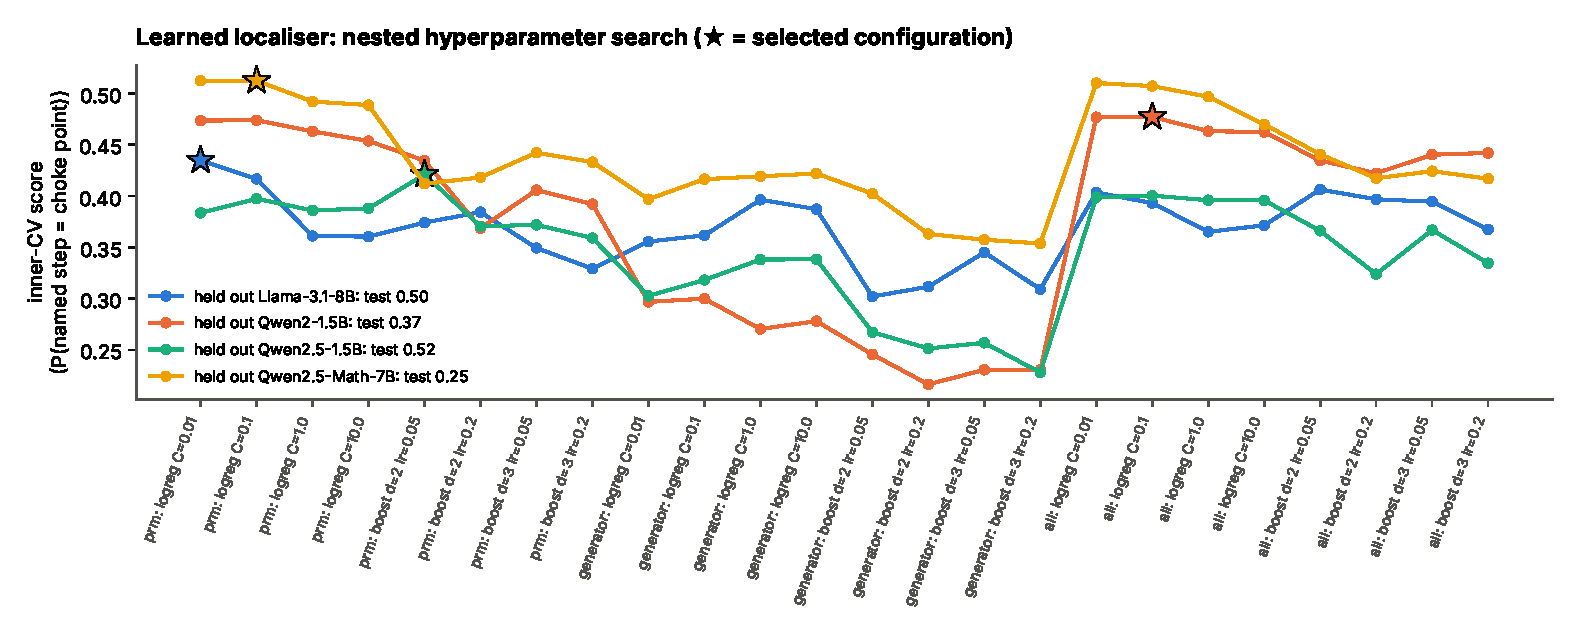
\includegraphics[width=\textwidth]{fig26_learned_tuning.pdf}
\caption{Nested hyperparameter search. One line per held-out model; stars mark the configuration
selected on the inner folds; the legend gives the score on the held-out model.}
\end{figure}

\begin{tabularx}{\linewidth}{lXcc}
\toprule
Held-out model & Selected features & Best inner score & Test score\\\midrule
Qwen2.5-1.5B & \ltQwenSmallFeat & \ltQwenSmallInner & \ltQwenSmallTest\\
Qwen2-1.5B & \ltQwenTwoFeat & \ltQwenTwoInner & \ltQwenTwoTest\\
Qwen2.5-Math-7B & \ltQwenMathFeat & \ltQwenMathInner & \ltQwenMathTest\\
Llama-3.1-8B & \ltLlamaFeat & \ltLlamaInner & \ltLlamaTest\\\bottomrule
\end{tabularx}

\textbf{What tuning taught us.} In three of the four outer folds the selection is a strongly
regularised logistic regression ($C=0.01$ or $0.1$), and in three of four it uses only the PRM
features: there is little transferable signal, so the search prefers simple models. Inner scores do not carry over to the held-out model (Qwen2.5-Math-7B:
\ltQwenMathInner\ inside, \ltQwenMathTest\ outside). The choke point is \emph{model-specific}; a
localiser tuned on some models does not transfer to a new one. Pooled, the tuned localiser finds the
choke point with probability \cbLearnedAccD, no better than the fixed PRM rule (\cbPrmDropAccD).

\subsection{4. A threshold tuned on DEV, tested on TEST (judge)}
For Part 3 we needed a grader that never reads a LettuceDetect score. The LLM judge flags a response
if it calls more than a fraction $f$ of its sentences unsupported. We chose $f$ from a grid fixed in
advance (0 to 0.5) by Cohen's $\kappa$ with human labels on the \robNDev\ DEV drafts and tested on
the \robNTest\ TEST drafts: $f^*=\robFstar\%$, TEST $\kappa=\robKEOneCal$.

\begin{caution}[The tuning mistake we caught]
The ``dual consensus judge'' added on 26 October had its threshold (0.3) chosen on \emph{all} 449
labelled drafts; the DEV/TEST split was introduced afterwards and then called ``out-of-sample''.
That is tuning on the test set. We withdrew the claim (Section~\ref{sec:integrity}). In the viva,
this is a good example of why the split must come before the choice.
\end{caution}

%==========================================================================================
\section{Results}\label{sec:results}
\begin{viva}[Research paper: Results (2.5 marks)]
Early warning reads difficulty (AUROC \aucQG\ from question + model); failures are often decided
before step 1; the human error is the choke point about half the time; PRMs find errors (\cbPrmDropAccHPct\%)
not choke points (\cbPrmDropAccDPct\%); restart is not beaten at matched compute (free oracle
\cbOracleGainB); the same in RAG (mechanism adds \rrHFive).
\end{viva}

\subsection{Mitigation: what works and what it costs}
\begin{tabularx}{\linewidth}{Xcccc}
\toprule
RAG mitigation (RAGTruth, 450 sources) & cost & $E_1$ & $E_2$ & coverage\\\midrule
No mitigation & 1.00$\times$ & \hallEOneBase & \hallETwoBase & \covBase\\
Delete flagged sentences & \costDel$\times$ & \hallEOneDel & \hallETwoDel & \covDel\\
\textbf{Detect, restart, abstain (DRA)} & \costDra$\times$ & \hallEOneDra & \hallETwoDra & \covDra\\
Claim repair, then delete & \costRep$\times$ & \hallEOneRep & \hallETwoRep & \covRep\\
CARE (choke-point-aware) & \costCare$\times$ & \hallEOneCare & \hallETwoCare & \covCare\\
Abstain on flagged QA & \costAbst$\times$ & \hallEOneAbst & \hallETwoAbst & \covAbst\\
Chain-of-Verification (raw, $n$=192) & \costCove$\times$ & \hallEOneCove & \hallETwoCove & \covCove\\\bottomrule
\end{tabularx}

Hallucination rates in \%. In maths, plain restarting solves \recMinOne--\recMaxOne\% of failed solutions
with one attempt, \recMinFour--\recMaxFour\% within four and \recMinEight--\recMaxEight\% within eight.
Human-scale prediction for DRA (Proposition 3): \lawH\% $\to$ \lawPi\% [\lawPiLo, \lawPiHi].

\textbf{Checking the law.} (1) Raising the retry budget from 1 to 4 on the same 450 sources raised
coverage from \invCovOne\% to \invCovFour\% while delivered hallucination moved by only \invETwo\
($E_2$) to \invEOne\ ($E_1$) points: retries buy coverage, not faithfulness, as predicted. (2) Sweeping
the detector threshold gives an operating curve: \ocDFivePi\% at \ocDFiveDraws\ generations per answer
(our setting) down to \ocUnionPi\% at \ocUnionDraws\ with a stricter gate (predicted from human labels).

\begin{figure}[h]\centering
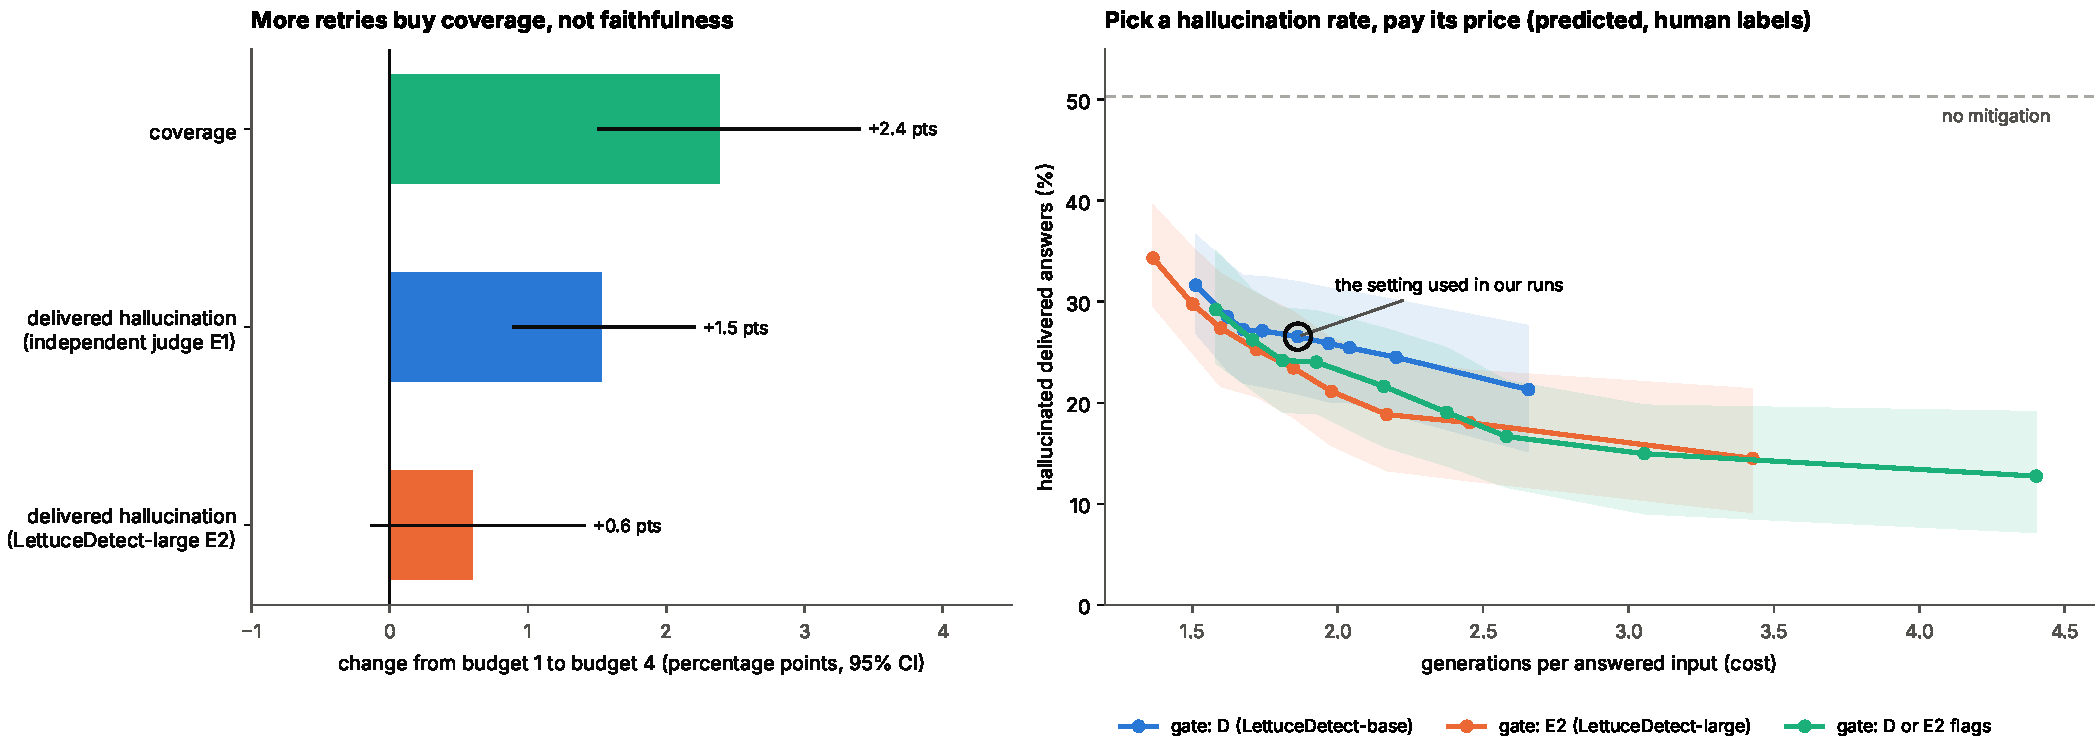
\includegraphics[width=\textwidth]{fig28_law.pdf}
\caption{Checks of Proposition 3: budget invariance (left) and the predicted operating curve (right).}
\end{figure}

\subsection{Part 1: early warning is a difficulty signal}
\begin{tabularx}{\linewidth}{Xc}
\toprule
Detector (out-of-fold, 3,400 traces) & AUROC\\\midrule
Question only & \aucQ\\
Generator and tier only & \aucG\\
Question + generator & \aucQG\ [\aucQGLo, \aucQGHi]\\
First 25\% of the reasoning only & \aucPA\\
Q + G + 25\% of the reasoning & \aucQGPA\ (increment \dIncA\ [\dIncALo, \dIncAHi])\\
Q + G + the whole reasoning & \aucQGPC\ (increment \dIncC)\\\bottomrule
\end{tabularx}

Within a problem, the 25\% prefix ranks failing above succeeding traces \wpPA\ of the time (chance is
0.5). \nonFatalPct\% of first errors are followed by a correct answer, and detectors rank these
non-fatal errors as \emph{riskier} than fatal ones (AUROC \twOutFR).

\subsection{Part 2: where failures are decided}
\begin{tabularx}{\linewidth}{Xcccc}
\toprule
 & Qwen2.5-1.5B & Qwen2-1.5B & Qwen2.5-Math-7B & Llama-3.1-8B\\\midrule
Decided before step 1 & \QwenSmallAllCapPct\% & \QwenTwoAllCapPct\% & \QwenMathCapPct\% & \LlamaCapPct\%\\
Human error = choke point & \QwenSmallAllDec & \QwenTwoAllDec & \QwenMathDec & \LlamaDec\\
\quad chance (position-matched) & \QwenSmallAllDecNull & \QwenTwoAllDecNull & \QwenMathDecNull & \LlamaDecNull\\
Restart $-$ backtrack to error, per attempt & \QwenSmallAllBtRestErr & \QwenTwoAllBtRestErr & \QwenMathBtRestErr & \LlamaBtRestErr\\\bottomrule
\end{tabularx}

\begin{itemize}
\item Reliability: $v_k$ from independent batches correlates at $r=\QwenSmallAllSplitR$ and
\QwenTwoAllSplitR; the most likely choke point has posterior probability $\ge 0.5$ in
\QwenSmallAllPostModal\% (Qwen2.5-1.5B) to \LlamaPostModal\% (Llama) of traces.
\item Preregistered on Llama: C3 (human error is the choke point more than chance) confirmed, Holm
$p$ \LlamaHolmCThree; C1 (restart beats backtracking to the error) \emph{not} confirmed
(\LlamaBtRestErr\ [\LlamaBtRestErrLo, \LlamaBtRestErrHi]). Replication on new batches (R1): \PooledNewBtRestErr\
[\PooledNewBtRestErrLo, \PooledNewBtRestErrHi], confirmed.
\end{itemize}

\subsection{Recovery policies at matched compute}
\begin{tabularx}{\linewidth}{Xcccc}
\toprule
P(solved) $-$ restart, budget 4 & Qwen2.5-1.5B & Qwen2-1.5B & Qwen2.5-Math-7B & Llama-3.1-8B\\\midrule
Restart: P(solved) & \QwenSmallPolRestartFour & \QwenTwoPolRestartFour & \QwenMathPolRestartFour & \LlamaPolRestartFour\\
PRM largest drop & \QwenSmallPolPrmDropFourDiff & \QwenTwoPolPrmDropFourDiff & \QwenMathPolPrmDropFourDiff & \LlamaPolPrmDropFourDiff\\
Learned restart point & \QwenSmallPolLearnedFourDiff & \QwenTwoPolLearnedFourDiff & \QwenMathPolLearnedFourDiff & \LlamaPolLearnedFourDiff\\
Human first error (not deployable) & \QwenSmallPolHumanFourDiff & \QwenTwoPolHumanFourDiff & \QwenMathPolHumanFourDiff & \LlamaPolHumanFourDiff\\\bottomrule
\end{tabularx}

The only positive estimate under full accounting: PRM largest drop on Qwen2.5-Math-7B at 8 attempts,
\QwenMathPolPrmDropEightDiff\ (exploratory).

\subsection{ChokeBench}
\begin{tabularx}{\linewidth}{Xcccc}
\toprule
Localiser & finds human error & finds choke point & $\Delta$/attempt & $\Delta$ at 4$\times$, free\\\midrule
Human first error & 1.00 & \cbHumanAccD & \cbHumanGain & \cbHumanGainB\\
PRM: largest drop & \cbPrmDropAccH & \cbPrmDropAccD & \cbPrmDropGain & \cbPrmDropGainB\\
PRM: first step $<0.5$ & \cbPrmFirstAccH & \cbPrmFirstAccD & \cbPrmFirstGain & \cbPrmFirstGainB\\
Learned, tuned & \cbLearnedAccH & \cbLearnedAccD & \cbLearnedGain & \cbLearnedGainB\\
Generator: max NLL & \cbNllAccH & \cbNllAccD & \cbNllGain & \cbNllGainB\\
Random step & \cbRandAccH & \cbRandAccD & \cbRandGain & \cbRandGainB\\\midrule
Oracle choke point & -- & -- & \cbOracleGain & \cbOracleGainB\ [\cbOracleGainBLo, \cbOracleGainBHi]\\\bottomrule
\end{tabularx}

\begin{figure}[h]\centering
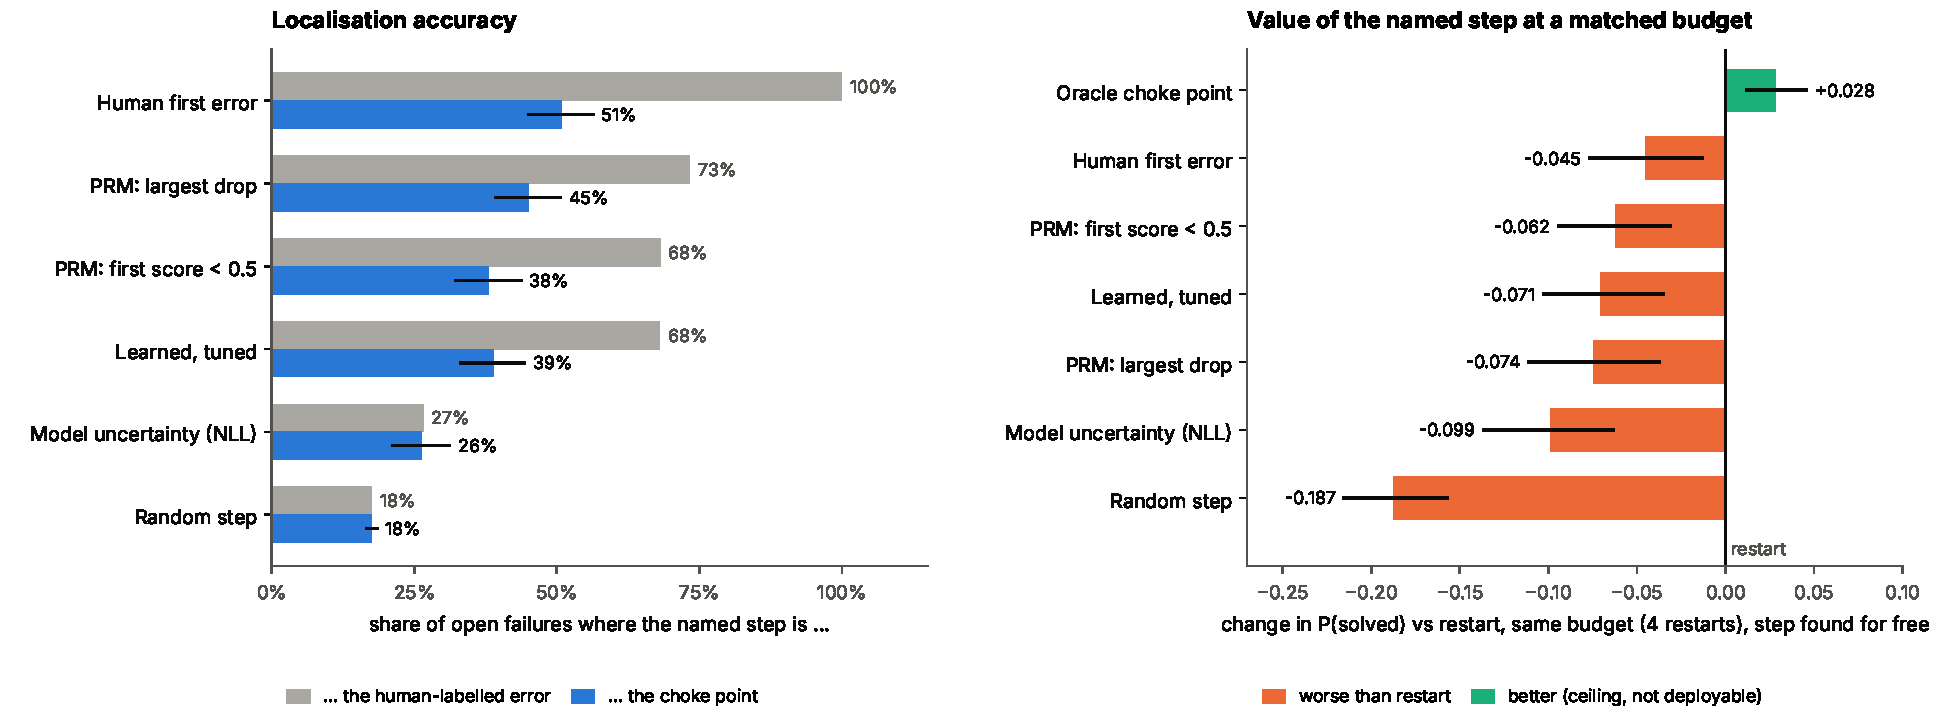
\includegraphics[width=\textwidth]{fig25_chokebench.pdf}
\caption{ChokeBench: localisation accuracy (left) and value of the named step at a matched budget (right).}
\end{figure}

\subsection{Part 3: hallucination recovery}
Preregistered (RAGTruth, judge $E_1$): CARE vs base \rrHZero\ [\rrHZeroLo, \rrHZeroHi] (supported);
CARE vs restart-until-$D$-passes \rrHOne\ (equivalent within $\pm0.03$; restart costs fewer tokens,
\rrRestartTok\ vs \rrCareTok); CARE vs its restart-only version \rrHFive\ [\rrHFiveLo, \rrHFiveHi].
Backtracking to just before the first human-marked hallucination vs restarting: \mechDiff\
[\mechDiffLo, \mechDiffHi]. No snowballing (\mechSnow).

Five graders, held-out half of RAGTruth (hallucination rate, \%):

\begin{tabularx}{\linewidth}{Xccccc}
\toprule
Policy & $E_1$ & $E_1$ calibrated & $E_2$ & dual & $D$\\\midrule
Base model & \robBaseEOne & \robBaseEOneCal & \robBaseETwo & \robBaseDual & \robBaseD\\
Restart until $D$ passes & \robRestartEOne & \robRestartEOneCal & \robRestartETwo & \robRestartDual & \robRestartD\\
CARE & \robCareEOne & \robCareEOneCal & \robCareETwo & \robCareDual & \robCareD\\
CoVe, revised answer & \robCoveEOne & \robCoveEOneCal & \robCoveETwo & \robCoveDual & \robCoveD\\\bottomrule
\end{tabularx}

The first two graders are independent of the gate $D$; the last three share its training data.

%==========================================================================================
\section{Result analysis: what the numbers mean}\label{sec:analysis}
\begin{viva}[Project: Result Analysis (5 marks)]
We read every result against a baseline, a null, an interval and a mechanism: Q+G for detectors,
a position-matched null for choke points, restart at matched compute for policies, a free oracle as
the ceiling, and an independent grader for RAG; and we explain the pattern with the supermartingale
argument.
\end{viva}

\subsection{Reading 1: why early warning looked good and is not}
A pooled AUROC of 0.588 sounds like the reasoning carries a warning signal. But hard problems fail
more often for every model, and the question text alone reveals difficulty. When the comparison is
\emph{within} one problem, the signal disappears (\wpPA). The counterfactual data explain why: for
\QwenSmallAllCapPct--\QwenMathCapPct\% of failures the model could not solve the problem from
scratch, so nothing in the reasoning could have changed the outcome.

\subsection{Reading 2: errors are not choke points}
The human-marked error is far more often the choke point than chance (e.g.\ Llama \LlamaDec\ vs
\LlamaDecNull), so labels are meaningful. But in the remaining traces either success had already
collapsed earlier (latent commitment) or the trace was still recoverable after the error. And
\nonFatalPct\% of first errors do not lead to a wrong answer at all. ``Where reasoning first goes
wrong'' and ``where the outcome is decided'' are different questions.

\subsection{Reading 3: verifiers learn the label they are trained on}
PRMs are trained and benchmarked on the human first error, and they find it well
(\cbPrmDropAccHPct\%). They find the choke point much less often (\cbPrmDropAccDPct\%). Training a
model directly for the choke point does not fix this (\cbLearnedAccD), and its tuning shows why: the
choke point depends on the generator, so features learned on some models do not transfer.

\subsection{Reading 4: why restart wins}
Three effects stack up.
\begin{enumerate}
\item \textbf{Theory.} Before the choke point a failed trace is, on average, worth no more than a fresh
start (supermartingale). Resampling from earlier in a failed trace keeps the parts that
already went wrong.
\item \textbf{The only real gain is saved tokens.} A later restart point means shorter continuations
and therefore more attempts in the same budget, about 15--29\% fewer tokens per attempt. That is
why even the perfect oracle gains only \cbOracleGainB.
\item \textbf{Verifiers cost compute.} A 7B PRM pass costs about five attempts of a 1.5B generator, so on
small models every verifier-based policy runs out of budget.
\end{enumerate}

\subsection{Reading 5: hallucinations behave the same way, and graders can fool you}
In RAG, resampling from before the first hallucinated sentence is not better than restarting, an
online recoverability estimate adds nothing, and a hallucinated sentence does not make the next ones
more likely. The more surprising lesson is about measurement. A loop that resamples until detector
$D$ is satisfied will look excellent to any grader that resembles $D$ (LettuceDetect-large agrees with
$D$ on \robAgreeETwoD\% of drafts): the gate is grading itself. The independent judge sees a much
smaller effect, but it agrees weakly with people, so neither number is the truth. Human ratings are
needed, and the blinded kit is ready.

\subsection{Reading 6: what to do in practice}
Under the graders we have (human ratings pending), the cheapest effective mitigation is to gate every output with a cheap detector, restart only what it
flags, and abstain or delete flagged sentences when the budget runs out. Proposition 3 says where
effort pays: the detector sets the hallucination rate of what is delivered, the budget sets how often
the system answers, and the resampling point sets neither. So a better detector is worth more than a
smarter repair.

\begin{plain}[The big picture]
Across maths and RAG, ``find the bad step and fix it'' is a natural idea that does not survive a
fair, compute-matched comparison against starting over. The useful levers are a better verifier
(to know \emph{whether} to retry) and an honest evaluator, not a smarter choice of \emph{where} to
retry.
\end{plain}

%==========================================================================================
\section{Mistakes we caught and corrected}\label{sec:integrity}
Being able to explain your own mistakes is a strength in a viva. These were found and fixed:
\begin{enumerate}
\item \textbf{Tie handling in AUROC} (original study): the lexical minus length-only gap at 25\% fell
from +0.073 to +0.052 ($p=0.032$) after correcting how tied scores were ranked.
\item \textbf{Chat preambles} (``Sure, here's the rewritten sentence:'') corrupted claim repairs; fixed in
parsing before the full run.
\item \textbf{Chain-of-Verification echo}: Llama-2 copied the verification Q\&A block into 89\% of its
answers, making CoVe look about 25 points worse than it is. Scoring only the revised answer fixes it.
\item \textbf{The dual consensus judge}: threshold chosen on all data, then called out-of-sample; and it
shares training data with the gate. Withdrawn.
\item \textbf{Llama-3.1 ``generalisation''}: reported detector flag rates as if they were failure rates;
no recovery policy was run on those outputs. Withdrawn; Llama-3.1 RAG drafts are kept as data only.
\item \textbf{Paper build}: the committed PDF predated Part 3, the source did not compile, and six
references had invented author lists. Rebuilt from the tables; references checked against arXiv and
ACL pages.
\item \textbf{Human-evaluation blinding}: the A/B key had been committed publicly. Removed; future kits
commit only its SHA-256 hash.
\end{enumerate}

%==========================================================================================
\section{Limitations and next steps}\label{sec:limits}
\begin{itemize}
\item Open models up to 8B parameters; maths for Parts 1--2, one generator for RAG.
\item ProcessBench solutions were re-segmented by its authors, so prefixes are near-, not exactly,
on-policy.
\item Llama-3.1-8B: 144 of 274 failed traces (GPU time limit); its RAG arm produced drafts only.
\item The independent RAG graders agree weakly with people; no human rating of system outputs yet.
\item ChokeBench and the learned localiser are exploratory, built from the same rollouts.
\end{itemize}
\textbf{Next:} (1) two human raters on the 80 blinded RAG pairs (regenerate the kit with a new seed
first); (2) the same protocol on long-reasoning models such as R1-distilled or Qwen3, where earlier
work finds prefixes can beat restarts, to find the boundary between the two regimes; (3) more
continuations per prefix on Llama.

%==========================================================================================
\section{Viva questions with short answers}\label{sec:qa}
\begin{description}[style=nextline]
\item[Q1. What is new in your work?] Not counterfactual resampling itself: Thought Anchors, Thought
Branches and \emph{The Point of No Return} use it, and Bulut (2026) compares prefixes with matched
restarts. What is new is comparing the counterfactual decision point with expert first-error labels,
on failed traces of four generators, and testing the recovery policies those labels motivate at
matched compute, with a bound that explains the result. ChokeBench packages this as a first
benchmark; RAG is a secondary application.
\item[Q2. Why not just train a bigger detector?] Because the limit is not the detector. Many failures
are decided before step 1, and even a perfect choke-point oracle gains only \cbOracleGainB.
\item[Q3. How do you know $v_k$ is not just noise?] Independent sampling batches agree ($r=\QwenSmallAllSplitR$),
Bayesian posteriors put the choke point clearly on one step in most traces, and the choke point is
chosen and scored on different halves of the samples.
\item[Q4. What is a position-matched null?] The share of traces where a randomly placed ``error'', with
the same position distribution as the real ones, would hit the choke point. It is about 0.16--0.20,
far below the observed 0.44--0.65.
\item[Q5. Why group by problem when splitting?] The same problem appears several times; a row split
would leak it into the test set and reward memorisation.
\item[Q6. Which hyperparameters did you tune, and how?] The learned localiser: \ltGrid\ configurations,
nested leave-one-generator-out CV. The judge threshold: grid on DEV, tested on TEST. Detector settings
were fixed in advance and checked across 5 seeds; $\delta$, $m$ and budget are reported as sensitivity.
\item[Q7. Why did the tuned model not beat the simple PRM rule?] The choke point is model-specific:
the best inner score (\ltQwenMathInner) dropped to \ltQwenMathTest\ on the held-out model. Little
transferable signal means regularised, simple models win and still do not beat a fixed rule.
\item[Q8. What does ``matched compute'' include?] Every prefill and generated token, PRM passes, probes and
oracle rollouts, weighted by model size, with the same budget for every policy.
\item[Q9. Explain the supermartingale argument simply.] On average over failures, the chance of success
at any point you pick without looking ahead is not higher than at the start; so backtracking cannot
beat restart per attempt unless it looks ahead or saves tokens.
\item[Q10. Which results failed?] C1 and C2 on Llama (backtracking to the human error is not worse than
restart for Llama), and every preregistered CARE comparison against an alternative strategy.
\item[Q11. Why is a negative result valuable?] It tells the field which baseline to beat. ``LLMs cannot
self-correct reasoning yet'' is a well-known example of a negative result that changed practice.
\item[Q12. Why do graders disagree in Part 3?] Restart-until-$D$-passes selects outputs that $D$ likes;
a grader trained on the same data likes them too. An independent grader sees much less.
\item[Q13. What is preregistration and why did you do it?] Writing hypotheses and analyses into git
before collecting data, so that results cannot be selected after the fact. Our commits
\texttt{a6fb04c} and \texttt{459ff22} predate the data they test.
\item[Q14. What would you do with more compute?] Human ratings for Part 3, and more continuations per cut
in Run D, to settle whether cheap late attempts really beat restart on reasoning models.
\item[Q15. So does your research reduce hallucination?] Not yet shown for people. Under the
preregistered LLM judge, detect--resample lowers the judged rate (\rrHZero, $p=\rrHZeroP$), but that
judge agrees only weakly with people ($\kappa=\evEOneKappa$) and flags 81\% of drafts where people
flag 50\%. The choke-point-aware controller is no better than plain restarting (\rrHOne) and costs
more (\costCare$\times$ against \costDra$\times$). Proposition~3 predicts \lawH\% $\to$ \lawPi\% for people, but
that is a prediction from human labels of drafts, not a measurement of outputs. The human rating
kit is the test.
\item[Q16. State and explain Proposition 3.] The loop returns the first answer the detector passes.
Each draw is passed-and-hallucinated with probability $h\beta$ or passed-and-faithful with
$(1-h)(1-\alpha)$, so a returned answer is hallucinated with probability $h\beta/(h\beta+(1-h)(1-\alpha))$
whatever the number of retries. Retries raise coverage, only the detector lowers hallucination.
\item[Q17. How did you test your own law?] It makes a falsifiable prediction: more retries should
raise coverage but not change the hallucination rate of delivered answers. From budget 1 to 4,
coverage rose by \invCov\ points and delivered hallucination moved by \invETwo\ to \invEOne\ points. A large
change would have refuted it.
\item[Q18. Can you beat Perplexity?] Not claimed. Perplexity is a web-search system judged on open-domain
factuality (SimpleQA); our task is faithfulness to given sources. The fair test is to run its API on the
same RAGTruth items and score it with the same graders, which we list as future work.
\item[Q19. Isn't this too many contributions for one paper?] It was, and a reviewer said so. We now
lead with one claim: human-labelled errors are not where failures are decided, and so localising
and repairing them does not beat restart at matched compute. The early-detection result is reported
as a negative result that motivates it, and the RAG study as a secondary application.
\item[Q21. Does ChokeBench predict which interventions work?] Yes, in our data, and without circularity.
One half of each prefix's samples labels the choke point and the other half scores the recovery gain,
so a hit cannot raise the gain mechanically. Within a trace, naming the choke point raises the gain
by \valBothD; the human label adds \valBothE\ once the choke point is accounted for. Across held-out
models, ChokeBench ranks localisers by gain with $\rho=\valRhoD$, against \valRhoE\ for first-error
scores. It is exploratory and on our own rollouts; outside replication is still needed.
\item[Q22. How will you show the hallucination reduction with people?] With a second blinded kit:
base model against detect--restart--abstain, on 80 of the 208 items where they differ, two raters,
key hash committed first. The planned analysis is fixed in its README.
\item[Q20. How can someone reproduce your numbers?] \texttt{make story} regenerates ChokeBench, the
grader analysis, the figures, every paper number and the PDF on a CPU in a few minutes; the GPU runs
have resumable Kaggle scripts.
\end{description}

\end{document}
